\chapter{Analiza modelu z zachowaniem stadnym}
\label{cha:spatial}

\section{Model matematyczny}

Model matematyczny opisujący zachowania ofiara-drapieżnik:

$$ \frac{\partial X}{\partial t} = rX(1-\frac{X}{K})-\frac{\alpha\sqrt{X}Y}{1+t_h \alpha\sqrt{X}}+d_x \bigtriangledown^2 X $$
$$ \frac{\partial Y}{\partial t} = sY^2+\frac{c\alpha\sqrt{X}Y}{1+t_h \alpha\sqrt{X}}+d_x \bigtriangledown^2 Y $$

gdzie 

\begin{eqwhere}[2cm]
	\item[$X$] liczebność populacji ofiary
	\item[$Y$] liczebność populacji drapieżnika
	\item[$r$] współczynnik przyrostu populacji ofiary
	\item[$K$] zdolność pojemnościowa układu
	\item[$\alpha$] efektywność poszukiwawcza populacji ofiar przez drapieżniki
	\item[$c$] współczynnik żarłoczności drapieżników
	\item[$t_h$] średni czas działania
	\item[$\frac{dx}{dt}$,$\frac{dy}{dt}$] współczynnik dyfuzji odpowiednich populacji
\end{eqwhere}

\noindent W powyższym modelu populacje poruszają się losowo - opisane poprzez model ruchów Browna. Zachowanie zostało uwzględnione w równaniach. Czas działania autor opracowania przyrównał do zera dla uproszczenia rozważań. $\bigtriangledown$ jest operatorem Laplace'a w przestrzeni dwuwymiarowej $R$ = ($R_1$,$R_2$) używanym dla wyrażenia ruchów populacji.

\section{Stabilność}

\noindent Interesuje nas stabilność tego systemu. Z biologicznego punktu widzenia jesteśmy zainteresowani w studiach zachowania koegzystujących populacji ofiar i drapieżnika. Niech punkt równowagi będzie postaci (x*,y*), gdzie obie populacje mają dodatnie wartości i żadna nie wymarła. Okazuje się, że takie ekwilibrium istnieje.

$$ x* = 1 - \frac{c}{s}, \quad y* = \frac{c}{s}\sqrt{x*}$$

\section{Bifurkacje}

\noindent Wraz ze zmianą niektórym parametrów (c,s) struktura jakościowa modelu może się dramatycznie zmienić. Bifurkacją nazywamy skokową zmianę właściwości modelu matematycznego przy niewielkiej zmianie parametrów. Przykładem może być liczba Reynoldsa, ważna w mechanice płynów bezwymiarowa liczba, która oszacowuje występujący podczas ruchu płynu stosunek sił bezwładności do sił lepkości. Przez zmianę tego parametru ruch płynu może zmienić się z laminarnego w falowy albo turbulentny.

\noindent W systemach reakcji-dyfuzji wyróżniamy dwa typy bifurkacji - Hopfa i Turinga. Interesującą bifurkacją jest ta druga, prowadzi bowiem do stanu, gdzie na całej modelowanej przestrzeni pojawiają wzory. W dwóch wymiarach są nimi zwykle heksagony lub figury o pasiastej aparycji.

\noindent W modelu możliwe jest wyznaczenie relacji między parametrem $s$ i $c$, dla którego wartość parametru $s$ będzie wartością krytyczną dla bifurkacji Hopfa i Turinga.

\begin{figure}[h]
	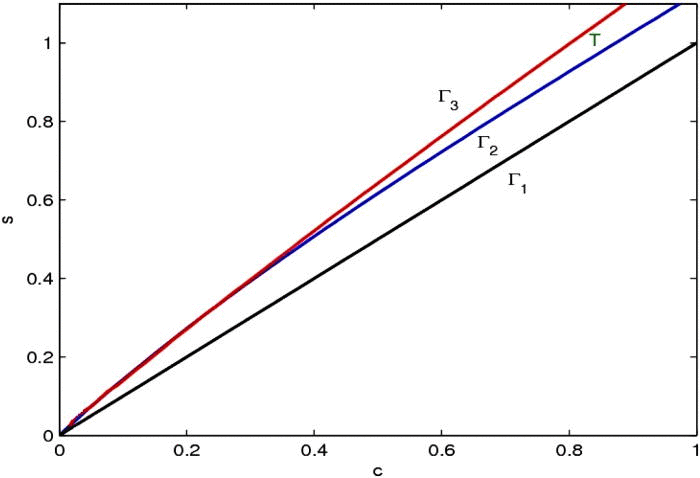
\includegraphics[width=\textwidth]{img/plane}
	\centering 
	\caption{Przestrzeń Turinga oznaczona jako T dla $\delta=10$. $\tau_1$,$\tau_2$,$\tau_3$ są kolejno są liniami bifurkacji Turinga, Hopfa, i ekwilibrium egzystencji.}
\end{figure}

\clearpage

\section{Symulacje}
\noindent Istotnie, interesujące zachowania ujawniają się dla wyznaczonych parametrów. Widoczne są różne kategorie wzorów na skutek bifurkacji Turinga dla różnych wartości parametrów w przestrzeni Turinga.


\begin{figure}[ht]
	\centering
	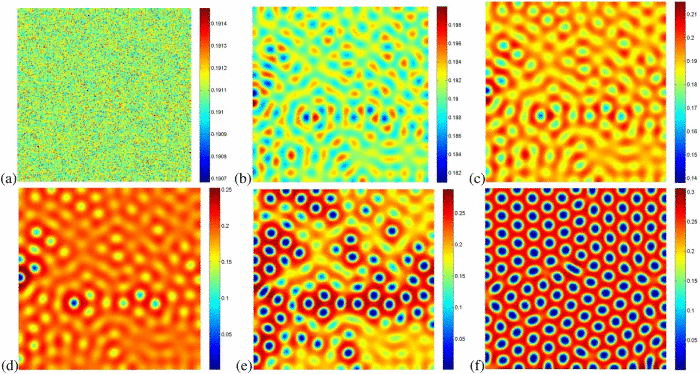
\includegraphics[width=0.6\textwidth]{img/3}
	
	\vspace*{\floatsep}% http://tex.stackexchange.com/q/26521/5764
	
	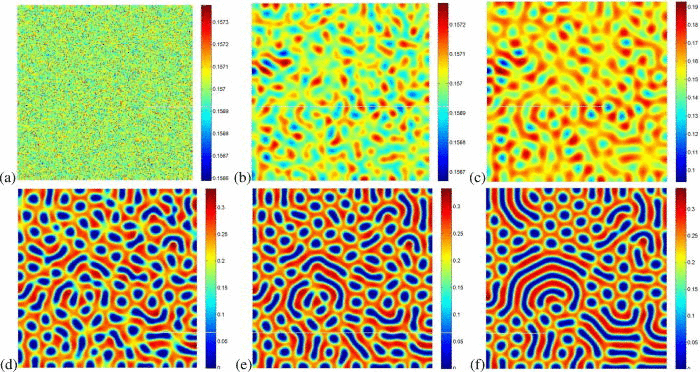
\includegraphics[width=0.6\textwidth]{img/2}
	
	\vspace*{\floatsep}% http://tex.stackexchange.com/q/26521/5764
	
	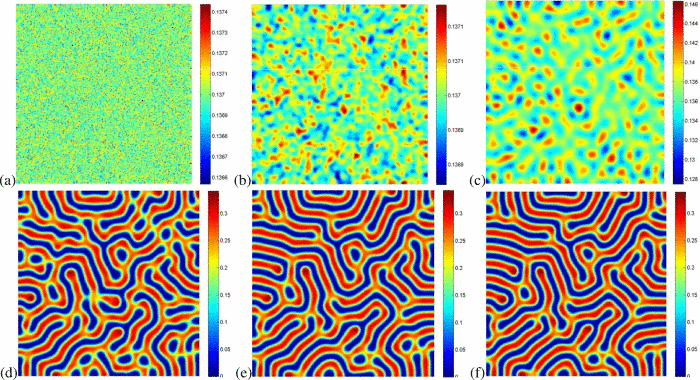
\includegraphics[width=0.6\textwidth]{img/1}
	
	\caption{Ewolucja zagęszczenia populacji ofiar w funkcji czasu}
\end{figure}

